%!TEX root = MS42.tex
\section{The Robot}\label{sec:therobot}
\subsection{KUKA LWR IV}

The robot used in the experimental platforms of PaCMan project is the \textit{KUKA Lightweight Robot IV} \cite{webkuka},  a 7-axis industrial manipulator which finds a wide employment in the field of the robotics research due to its flexibility and modularity, including a payload capacity of 7 Kg. In addition, the seventh axis makes the robot redundant, which mean that, for a given position and orientation of the end effector, there exist multiple configurations in the joints space. Each joint is equipped with a position and a torque sensor, allowing the robot to be operated with position, velocity and torque control. 

\begin{figure}[h]
\centering
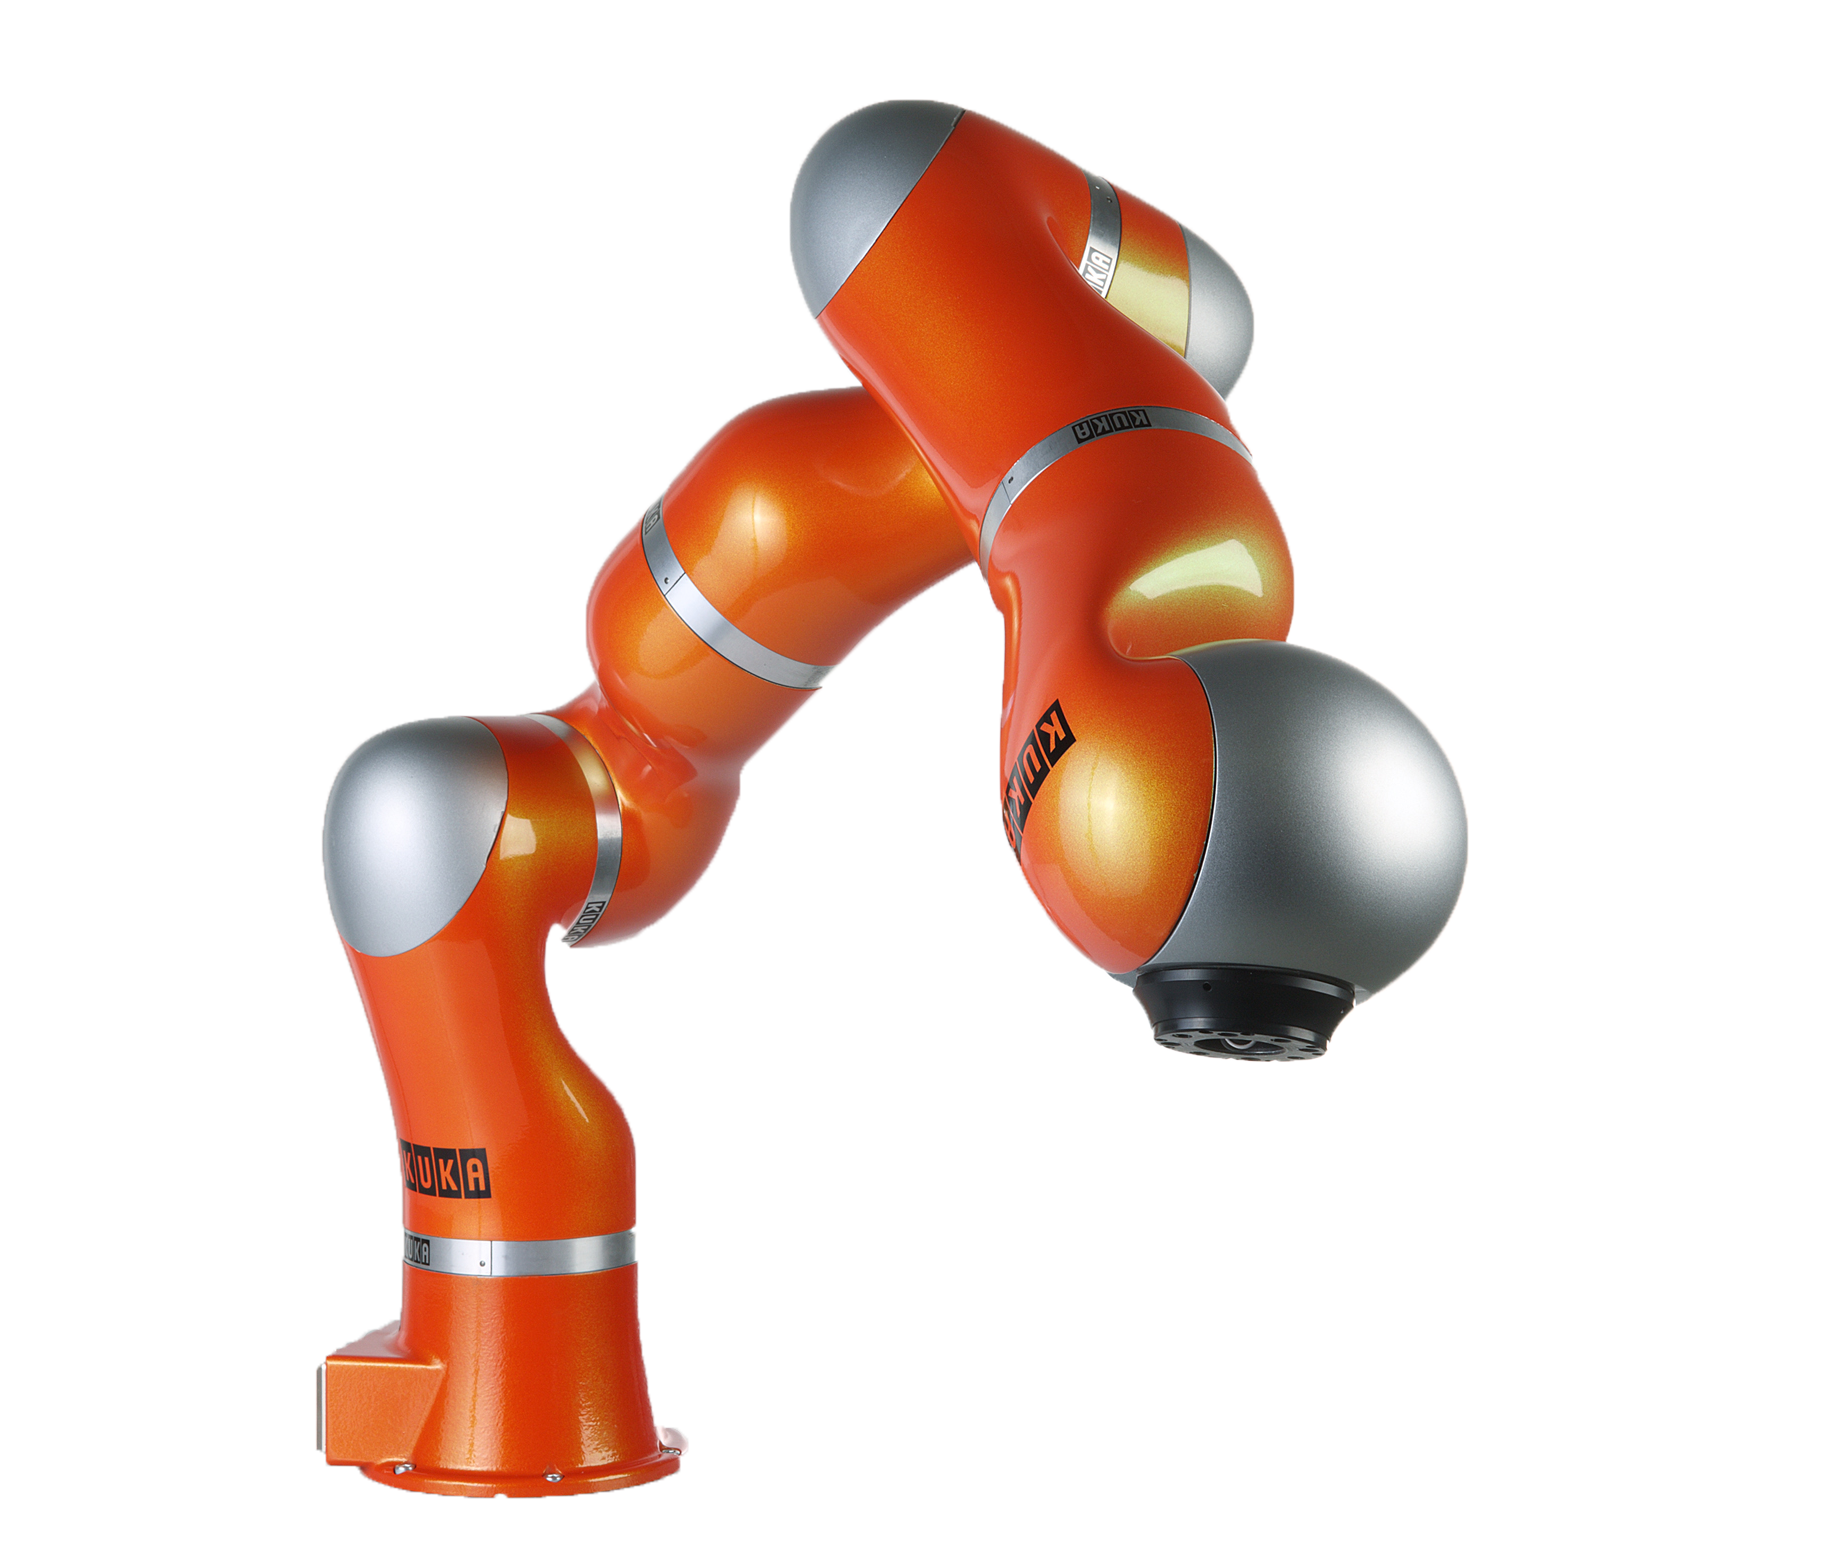
\includegraphics[scale=0.7]{kuka}
\caption{KUKA Lightweight Robot IV arm}
\end{figure}

The communication between the robot and an external computer is handled by the \textit{Fast Research Interface} (FRI), a real-time proprietary software interface able to read and write system variables of the robot and execute user-programs.

\subsection{Built-in Control Strategies}
The robot provides three different control strategies as default setting, which are described below \cite{kukafri}.
\subsubsection*{Position Controller}
The position controller takes as command the desired joints set-point position, ensuring regulation through the use of an internal \textit{PID}. 

\subsubsection*{Cartesian Stiffness Controller}
The Cartesian stiffness controller is characterized by the following control law:
\begin{equation}
\tau_{cmd} = J^T(k_c(x_{FRI} - x_{msr}) + F_{FRI}) + D(d_c) + f_{dynamics}(q,\dot{q},\ddot{q})
\label{eq:cartesianstiffnesscontroller}
\end{equation}
where:
\begin{itemize}
\item $\tau_{cmd}\in\mathbb{R}^7$: control torque;
\item $x_{FRI}\in\mathbb{R}^{12}$: commanded cartesian set-point position;
\item $x_{msr}\in\mathbb{R}^{12}$: measured cartesian position;
\item $k_c\in\mathbb{R}^{7\times 7}$: cartesian stiffness;
\item $D(d_c)\in\mathbb{R}^7$: damping term;
\item $f_{dynamics}(q,\dot{q},\ddot{q})\in\mathbb{R}^7$: the dynamic compensation;
\item $F_{FRI}\in\mathbb{R}^7$: the cartesian external force.
\end{itemize}

\subsubsection*{Axis-specific Stiffness Controller}
The axis-specific stiffness controller is similar to the cartesian stiffness controller, but it takes commands in joints space:
\begin{equation}
\tau_{cmd} = k_j(q_{FRI} - q_{msr}) + D(d_j) + \tau_{FRI} + f_{dynamics}(q,\dot{q},\ddot{q})
\label{eq:axisspecificstiffnesscontroller}
\end{equation}
where:
\begin{itemize}
\item $\tau_{cmd}\in \mathbb{R}^7$: control torque;
\item $q_{FRI}\in\mathbb{R}^7$: commanded joint set-point position;
\item $q_{msr}\in\mathbb{R}^7$: measured joint position;
\item $k_j\in\mathbb{R}^{7\times 7}$: joint stiffness;
\item $D(d_j)\in\mathbb{R}^7$: damping term;
\item $f_{dynamics}(q,\dot{q},\ddot{q})\in\mathbb{R}^7$: the dynamic compensation;
\item $\tau_{FRI}\in\mathbb{R}^7$: the joint external force.
\end{itemize}
\newpage